\section{Methodology}

\subsection{Problem Definition}
\label{sec:problem}

\begin{definition}[Variation graph]
A variation graph $G=(V,E,\sigma,\mathcal{P})$ is a directed acyclic graph whose nodes carry sequence labels $\sigma:V\to\Sigma^{+}$, $\Sigma=\{\mathrm{A,C,G,T}\}$, and whose haplotypes are the source-to-sink paths in $\mathcal{P}$. A snarl $S=(s,t)$ is a minimal pair of boundary nodes that separates the subgraph between them from the rest of $G$ \cite{paten2018superbubbles}; snarls nest into a snarl tree $T(G)$. An allele of $S$ is an $s\!\to\!t$ path, read as the concatenated labels of its interior nodes; $\mathcal{A}(S)$ is the set of alleles of $S$ and $k=|\mathcal{A}(S)|$.
\end{definition}

\begin{definition}[Graph-to-graph alignment]
Given variation graphs $G_A,G_B$ with labels $\sigma_A,\sigma_B$, an alignment $\mathcal{M}=(M_v,M_e,M_s)$ consists of partial one-to-one maps between their nodes, edges and snarls such that (i)~$M_s$ preserves ancestry between $T(G_A)$ and $T(G_B)$ and the order of snarls along the matched backbone $M_v$, and (ii)~each snarl pair $(S,S')\in M_s$ carries a partial one-to-one allele matching $\mu_{S,S'}\subseteq\mathcal{A}(S)\times\mathcal{A}(S')$. The problem is to find $\mathcal{M}^{\ast}=\arg\max_{\mathcal{M}}W(G_A,G_B,\mathcal{M})$, where
\begin{align}
W(G_A,G_B,\mathcal{M}) =\;
&\alpha\!\!\sum_{(u,v)\in M_v}\!\!\mathrm{sim}(\sigma_A(u),\sigma_B(v))
+\beta\!\!\sum_{(e,e')\in M_e}\!\!\mathbf{1}[\text{cons.}] \nonumber\\
&+\gamma\!\!\sum_{(S,S')\in M_s}\!\!\mathrm{SimBubble}(S,S'),
\label{eq:score}
\end{align}
$\mathrm{sim}(s_1,s_2)=1-\mathrm{edit}(s_1,s_2)/\max(|s_1|,|s_2|)$, $\mathbf{1}[\text{cons.}]$ indicates that a matched edge joins matched endpoints, and $\mathrm{SimBubble}(S,S')$ is the summed similarity of the allele pairs in $\mu_{S,S'}$ minus a gap penalty per unmatched allele. The output is the delta graph $\Delta_{A\to B}$ (resp.\ $\Delta_{B\to A}$), the alleles of $G_A$ (resp.\ $G_B$) left unmatched by $\mathcal{M}^{\ast}$, including every allele of a snarl without partner, and the shared alignment induced by the matched elements.
\end{definition}

Condition~(i) separates this problem from general graph matching: without it the problem contains subgraph isomorphism and is NP-hard \cite{GUPTA1996287}; with it the optimum decomposes over the snarl tree \eqref{eq:dp} and every leaf is an assignment problem. PanG2G solves each allele matching $\mu$ exactly and the snarl map $M_s$ heuristically (\S\ref{sec:algo}), so it returns a feasible alignment whose within-snarl part is optimal but which need not equal $\mathcal{M}^{\ast}$. In the reference-anchored mode (\S\ref{sec:refdiff}), $M_s$ is instead fixed by shared reference coordinates and alleles match only when identical.

\subsection{The Algorithm}
\label{sec:algo}
PanG2G has five stages (Fig. \ref{fig:pipeline}): (1) detect anchors, nodes shared by both graphs; (2) decompose each graph into its snarl tree; (3) pair snarls across the graphs; (4) run a per-snarl-pair dynamic program whose leaf operation is allele matching; (5) emit the delta graphs $\Delta_{A\to B},\Delta_{B\to A}$ (Fig. \ref{fig:delta}), the shared alignment, and a global score.

The formulation supports the nested recurrence \eqref{eq:dp}, but the implementation and evaluation are depth-1: nested snarls are detected but only top-level snarls are kept, each with its $s\!\to\!t$ paths as alleles, and the graphs we evaluate (vg construct and synthetic generators) contain only simple SNP/indel bubbles; this paper reports no results on nested Minigraph-Cactus graphs. The recurrence, the van~Emde~Boas layout and the DAG dependencies are therefore exercised only at depth~1, where they reduce to independent per-snarl-pair assignments, and the numbers in \S\ref{sec:eval} should be read with this scope in mind. In \eqref{eq:score}, $(\alpha,\beta,\gamma)$ default to $(1,0.5,2)$: the structural term is up-weighted because allele identity is the primary delta signal, and we do not sweep them because the delta depends only on the within-snarl matching $\mu$, whose ranking of allele pairs is invariant to $\gamma$'s scale. Sibling snarls are separated by their boundary nodes, so their subproblems are independent and each depth-1 pair is one $O(k^3)$ bipartite matching.

\begin{figure}[t]
  \centering
  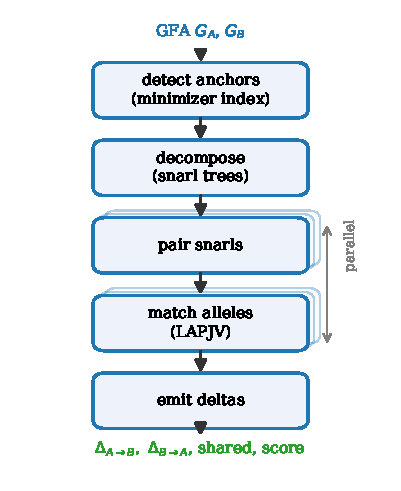
\includegraphics[width=0.55\columnwidth]{figs/fig_pipeline.pdf}
  \caption{The PanG2G pipeline. (1)~Detect anchors via a minimizer index. (2)~Decompose each graph into its snarl tree. (3)~Pair snarls by boundary key (default) or anchor-interval dynamic programming. (4)~Match alleles within each pair by LAPJV assignment. (5)~Emit the delta graphs, the shared alignment (GAF-style) and a global score. Stage 4 runs in parallel (faded copies) under the priority-dispatch scheduler.}
  \label{fig:pipeline}
\end{figure}

\begin{algorithm}[t]
\caption{PanG2G alignment (\textbf{depth-1 form}, as implemented and evaluated). Each snarl pair is an independent leaf solved by one $O(k^3)$ assignment. $W_{\text{seq}}=\alpha\cdot$ mean similarity of the two snarls' source and sink nodes; $W_{\text{topo}}=\beta\cdot\mathbf{1}[\text{both are simple bubbles}]$. The shared alignment $H$ (anchors, snarl pairs and their allele matchings) is written as a GAF-style alignment file, not materialized as a graph.}
\label{alg:g2g}
\begin{algorithmic}[1]
\Require graphs $G_A,G_B$; weights $\alpha,\beta,\gamma$; gap $g$; floor $\tau$
\Ensure deltas $\Delta_{A\to B},\Delta_{B\to A}$, shared alignment $H$, score $W$
\State $\mathcal{N}\gets \Call{FindAnchors}{G_A,G_B}$ \Comment{minimizer index}
\State $T_A\gets\Call{Decompose}{G_A}$;\ $T_B\gets\Call{Decompose}{G_B}$ \Comment{superbubbles}
\State $P\gets\Call{PairSnarls}{T_A,T_B,\mathcal{N}}$ \Comment{boundary key or anchor-interval DP}
\State $\mathcal{T}\gets\Call{BuildTaskDAG}{P}$ \Comment{priority $=\sum k_i^3$}
\ParFor{$(S_A,S_B)\in\mathcal{T}$ \textbf{by priority dispatch}}
   \State $a\gets\Call{Alleles}{S_A}$;\ $b\gets\Call{Alleles}{S_B}$
   \State $C_{ij}\gets 1-\mathrm{sim}(a_i,b_j)$; clamp $C_{ij}\!>\!1{-}\tau$ to $g$
   \State $(s,\mu)\gets\Call{LAPJV}{C}$ \Comment{$O(k^3)$ assignment}
   \State $w[S_A,S_B]\gets W_{\text{seq}}+W_{\text{topo}}+\gamma\,s$; record $\mu$
\EndParFor
\State $W\gets\!\sum w[S_A,S_B]+\alpha\!\!\sum_{(u,v)\in\mathcal N}\!\!\mathrm{sim}(u,v)$
\State $U_A,U_B\gets$ alleles unmatched by the $\mu$'s $\cup$ alleles of unpaired snarls
\State $\Delta_{A\to B},\Delta_{B\to A}\gets\Call{BuildDeltas}{U_A,U_B}$
\State $H\gets\mathcal{N}\cup P\cup\{\mu\}$ \Comment{shared alignment}
\State \Return $\Delta_{A\to B},\Delta_{B\to A}$, $H$, $W$
\end{algorithmic}
\end{algorithm}

With nested children the score decomposes recursively,
\begin{equation}
\mathrm{OPT}(S_A,S_B)=W_{\text{seq}}+W_{\text{topo}}+\max_{\mu}\sum_{(c,c')\in\mu}\mathrm{OPT}(c,c'),
\label{eq:dp}
\end{equation}
with $\mu$ over child-snarl matchings and the leaf case reducing to Algorithm~\ref{alg:g2g}; the implementation processes children before parents in van~Emde~Boas post-order, a path that is inert at depth~1 (confirmed by the vEB ablation, Fig. \ref{fig:ablation}).

\subsubsection{Anchor detection}
Anchors are node pairs with in- and out-degree $\le 1$ in both graphs whose sequences are near-identical ($\mathrm{sim}\ge0.9$); the degree rule admits the invariant backbone chain between bubbles and also the allele nodes of simple bubbles, so shared alleles act as anchors too. A naive all-pairs scan is quadratic (${\sim}10^{14}$ comparisons at human scale, $|V|\sim10^7$); PanG2G instead builds a minimizer index \cite{li2018minimap2} over one graph's eligible nodes: candidate pairs share a minimizer, are refined by full similarity and resolved greedily, and nodes shorter than the $k$-mer length (15\,bp) produce no minimizer and are never anchored. On the vg~construct graphs of \S\ref{sec:eval}, half of all nodes satisfy the degree rule but over 80\% of them are 1-bp SNP alleles, so anchors come from the ${\sim}15\%$ of eligible nodes of ${\ge}15$\,bp, the reference chunks between variants (vg construct chops invariant sequence into nodes of at most 32\,bp). Anchors contribute the $\alpha$ term of \eqref{eq:score}; the default pairing does not use them, and only the anchor-interval pairing below uses them to pin the two coordinate systems together. Anchoring is one-to-one, so differently cut nodes are not anchored; the reference-anchored mode (\S\ref{sec:refdiff}), which keys variants by coordinate, is unaffected.

\subsubsection{Snarl decomposition and pairing}
PanG2G can take snarl boundaries from \texttt{vg snarls} \cite{garrison2018vg} (optional backend), but by default uses a built-in superbubble scan after Onodera et al.\ \cite{onodera2013superbubbles}, restricted to DAGs: from each branching node the scan walks the topological order, admitting a node once all its predecessors are visited, and closes the snarl at the first node that is the only frontier node left. Each scan costs the size of its bubble, so the decomposition is near-linear on bubble chains ($N^{1.00}$, Fig.~\ref{fig:refdiffscaling}). Both backends then enumerate every $s\!\to\!t$ path as an allele. Snarls are paired by their boundary key: two snarls correspond when the sequences of their source and sink nodes are identical, and repeated keys are consumed in topological order (FIFO). This rule is $O(|T_A|+|T_B|)$ and exact when keys are unique, but a snarl present in only one graph whose key repeats shifts every later snarl with that key by one position; on vg~construct graphs 10--13\% of bubbles share their key with another bubble, because 35--40\% of boundary nodes are ${\le}2$\,bp. PanG2G therefore also offers an anchor-interval pairing (\texttt{--pairing interval}): anchors are chained in topological order and the snarls between two consecutive anchors are paired by an order-preserving dynamic program (a Needleman-Wunsch over the two snarl sequences) whose match score is the fraction of identical allele sequences plus the boundary similarity. An error can then not cross an anchor and the pairing is optimal within each interval; the cost is $\sum_i|A_i|\,|B_i|$ over intervals, near-linear when anchors are dense. Both rules are compared in \S\ref{sec:eval} (Q1). Unpaired snarls in either graph send all their alleles to that graph's delta.

\subsubsection{Per-snarl bipartite matching}
Within a paired snarl we want the maximum-similarity partial allele matching, with unmatched alleles paying a gap cost. PanG2G builds the $k\times k$ cost matrix $C_{ij}=1-\mathrm{sim}(a_i,b_j)$, clamps pairs below a similarity floor ($\tau=0.75$) to the gap cost so the solver prefers a gap over a bad match, pads rectangular instances with gap-cost dummies, and solves the assignment exactly with Jonker-Volgenant in $O(k^3)$ \cite{jonker1987shortest}, so one pass optimizes matches and gaps jointly. For rare very large snarls ($k>30$) a greedy $1/2$-approximation is available as a fallback; a brute-force routine is retained only as a $k\le 8$ oracle.

\subsubsection{The output}
The delta graph $\Delta_{A\to B}$ lists every allele present in $A$ but unmatched in $B$ (and symmetrically for $\Delta_{B\to A}$): the population-specific variants (Fig. \ref{fig:delta}), each with its exact inserted/deleted sequence. This is the graph-level analogue of a VCF, which no sequence-to-reference pipeline can produce without first collapsing both graphs onto a shared linear backbone.

\begin{figure}[t]
  \centering
  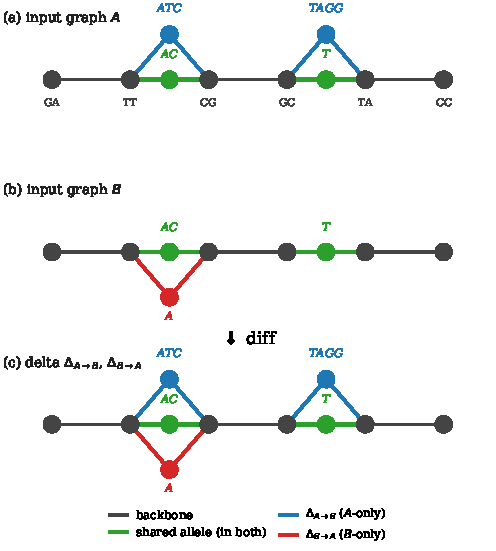
\includegraphics[width=0.7\linewidth]{figs/fig_delta.pdf}
  \caption{The delta at base-pair resolution; every circle is a node storing a
  string of base pairs. Input graphs (a)~$A$ and (b)~$B$ share
  an allele (green) at each snarl and add their own alternative (blue for $A$,
  red for $B$). (c)~the delta keeps the alleles in exactly one graph:
  $\Delta_{A\to B}$ (blue) and $\Delta_{B\to A}$ (red), each with its exact
  sequence.}
  \label{fig:delta}
\end{figure}


\subsection{Workload Profiling}
\label{sec:workload}

Before building the parallel engine we profiled the reference prototype on synthetic graphs whose snarl sizes follow a Zipf law fit to HPRC statistics.

\textbf{Finding 1: matching cost explodes with snarl size.}
Fig. \ref{fig:workload}b shows measured time per snarl pair as a function of allele count $k$. Brute-force enumeration ($O(k!)$) is fast for SNP bubbles but becomes infeasible beyond $k{\approx}8$ (57\,ms per pair at $k{=}8$ in C++, 2\,s in the Python prototype). The $O(k^3)$ LAPJV solver flattens this curve (1.2\,ms at $k{=}50$) and is what makes complex structural-variant regions tractable, where $k$ can reach 20-50 \cite{jonker1987shortest}.

\textbf{Finding 2: the workload is heavy-tailed and scale-invariant.}
Most snarls are tiny ($67\%$ are $k{=}2$ SNP bubbles) but a few are much larger, so per-snarl work ($\propto k^3$) is highly skewed. The Gini coefficient of work stays in the narrow band $0.55$-$0.58$ across graph sizes spanning $20$ to $1000$ snarls (Fig. \ref{fig:workload}a; $k\le6$ in the prototype profiling): the imbalance does not wash out with scale. Real graphs have $10^6$-$10^7$ snarls, so this is suggestive, not a deployment-scale demonstration. A static, equal-count partition of snarls across threads would be badly load-imbalanced, because a handful of large snarls dominate the work; this mandates a priority-dispatch scheduler.

\begin{figure}[t]
  \centering
  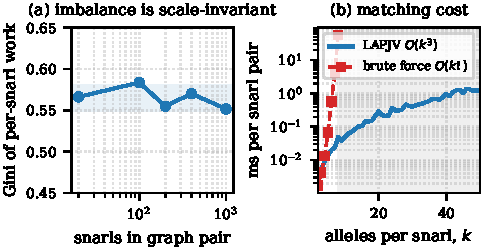
\includegraphics[width=\linewidth]{figs/fig_workload_matching.pdf}
  \caption{(a)~The Gini coefficient of per-snarl work stays above $0.55$ across graph sizes (reference prototype, HPRC-calibrated synthetic graphs): the heavy tail is scale-invariant, so static partitioning is load-imbalanced at every scale. (b)~Measured cost of the per-snarl bipartite matching versus allele count $k$ (C++ engine, 12-bp alleles, mean of 20 pairs); brute force is infeasible beyond $k{=}8$.}
  \label{fig:workload}
\end{figure}

\textbf{Finding 3: memory access, not arithmetic, is the scaling wall.}
The snarl tree is traversed bottom-up and each snarl-pair dynamic program (DP) reads allele sequences from both graphs. At human scale the working set exceeds DRAM for a naive layout, which points to a cache-friendly layout for the snarl tree and to flat, contiguous sequence storage rather than pointer-chasing per-node strings.

\subsection{System Design and Implementation}
\label{sec:system}

PanG2G is implemented in C++20 with a Python reference prototype as a correctness oracle (the prototype pairs snarls greedily by score over all pairs, which is quadratic; the engine uses the linear rules above). Graphs are read from GFA\,v1.1 (S/L/P and W lines, with on-the-fly reverse complementing). All node sequences live in one flat byte array indexed by (offset, length) and adjacency in CSR form, so the DP kernel streams sequence data without pointer chasing. Experiments run on a single-socket AMD EPYC 7763 (Milan): 64 cores, 4 NUMA domains, 512 GiB DDR4-3200, 256 MiB L3; Ubuntu 20.04, GCC 9.4 -O3, except where a laptop is named.

\textbf{Cache-oblivious snarl-tree layout.}
Each snarl's DP table and allele data sit contiguously in one arena block, which helps on all workloads and is always on. On a nested tree, breadth-first storage scatters sibling subtrees, so a bottom-up traversal thrashes the cache once the working set exceeds L3; PanG2G instead lays the tree out in van Emde Boas order \cite{vanemde1977preserving,frigo1999cache}, storing any size-$S$ subtree in $O(S/B)$ contiguous lines, so a bottom-up traversal is scan-optimal at $O(N/B)$ misses. All evaluated trees have depth~1, where vEB order $\equiv$ BFS order; the feature is implemented for the nested Minigraph-Cactus graphs that are the deployment target.

\textbf{Centralized priority-dispatch runtime.}
Motivated by Finding 2, the snarl-pair DP is a shallow task DAG scheduled with Longest-Processing-Time-first (LPT) list scheduling \cite{graham1969bounds} on OpenMP: a single mutex-guarded priority queue keyed on estimated subtree work ($\sum k_i^3$), from which idle workers pop the largest task. We chose one shared queue over per-thread work-stealing deques because randomized stealing loses the largest-first property LPT relies on; lock contention did not limit scaling up to 128 physical cores, and chunked dispatch made it worse (\S\ref{sec:eval}, Q2). The parallel delta is byte-identical to the sequential aligner's and the score agrees to $10^{-3}$, float-order aside.

\textbf{Exact matching and anchor index.}
The solver is a self-contained Jonker-Volgenant implementation \cite{jonker1987shortest}: the dispatcher routes $k\le 30$ to LAPJV and larger snarls to the greedy fallback. The minimizer anchor index uses FNV-1a hashing over $k$-mers with a minimap2-style window \cite{li2018minimap2}, a build-time toggle against the naive scan.
